% Created by tikzDevice version 0.12.3.1 on 2021-12-06 11:02:57
% !TEX encoding = UTF-8 Unicode
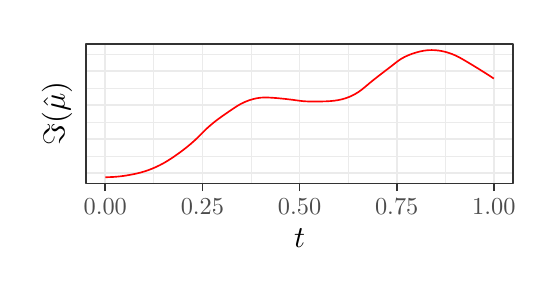
\begin{tikzpicture}[x=1pt,y=1pt]
\definecolor{fillColor}{RGB}{255,255,255}
\begin{scope}
\definecolor{drawColor}{RGB}{255,255,255}
\definecolor{fillColor}{RGB}{255,255,255}

\path[draw=drawColor,line width= 0.6pt,line join=round,line cap=round,fill=fillColor] (  0.00,  0.00) rectangle (180.67, 86.72);
\end{scope}
\begin{scope}
\definecolor{fillColor}{RGB}{255,255,255}

\path[fill=fillColor] ( 20.71, 30.69) rectangle (175.17, 81.22);
\definecolor{drawColor}{gray}{0.92}

\path[draw=drawColor,line width= 0.3pt,line join=round] ( 20.71, 40.66) --
	(175.17, 40.66);

\path[draw=drawColor,line width= 0.3pt,line join=round] ( 20.71, 52.95) --
	(175.17, 52.95);

\path[draw=drawColor,line width= 0.3pt,line join=round] ( 20.71, 65.24) --
	(175.17, 65.24);

\path[draw=drawColor,line width= 0.3pt,line join=round] ( 20.71, 77.53) --
	(175.17, 77.53);

\path[draw=drawColor,line width= 0.3pt,line join=round] ( 45.29, 30.69) --
	( 45.29, 81.22);

\path[draw=drawColor,line width= 0.3pt,line join=round] ( 80.39, 30.69) --
	( 80.39, 81.22);

\path[draw=drawColor,line width= 0.3pt,line join=round] (115.50, 30.69) --
	(115.50, 81.22);

\path[draw=drawColor,line width= 0.3pt,line join=round] (150.60, 30.69) --
	(150.60, 81.22);

\path[draw=drawColor,line width= 0.6pt,line join=round] ( 20.71, 34.52) --
	(175.17, 34.52);

\path[draw=drawColor,line width= 0.6pt,line join=round] ( 20.71, 46.81) --
	(175.17, 46.81);

\path[draw=drawColor,line width= 0.6pt,line join=round] ( 20.71, 59.09) --
	(175.17, 59.09);

\path[draw=drawColor,line width= 0.6pt,line join=round] ( 20.71, 71.38) --
	(175.17, 71.38);

\path[draw=drawColor,line width= 0.6pt,line join=round] ( 27.74, 30.69) --
	( 27.74, 81.22);

\path[draw=drawColor,line width= 0.6pt,line join=round] ( 62.84, 30.69) --
	( 62.84, 81.22);

\path[draw=drawColor,line width= 0.6pt,line join=round] ( 97.94, 30.69) --
	( 97.94, 81.22);

\path[draw=drawColor,line width= 0.6pt,line join=round] (133.05, 30.69) --
	(133.05, 81.22);

\path[draw=drawColor,line width= 0.6pt,line join=round] (168.15, 30.69) --
	(168.15, 81.22);
\definecolor{drawColor}{RGB}{255,0,0}

\path[draw=drawColor,line width= 0.6pt,line join=round] ( 27.74, 32.98) --
	( 29.14, 33.01) --
	( 30.54, 33.07) --
	( 31.95, 33.18) --
	( 33.35, 33.32) --
	( 34.76, 33.51) --
	( 36.16, 33.74) --
	( 37.56, 34.00) --
	( 38.97, 34.29) --
	( 40.37, 34.63) --
	( 41.78, 35.04) --
	( 43.18, 35.50) --
	( 44.59, 36.04) --
	( 45.99, 36.64) --
	( 47.39, 37.31) --
	( 48.80, 38.05) --
	( 50.20, 38.88) --
	( 51.61, 39.78) --
	( 53.01, 40.73) --
	( 54.41, 41.72) --
	( 55.82, 42.76) --
	( 57.22, 43.86) --
	( 58.63, 45.03) --
	( 60.03, 46.27) --
	( 61.44, 47.59) --
	( 62.84, 49.02) --
	( 64.24, 50.42) --
	( 65.65, 51.68) --
	( 67.05, 52.84) --
	( 68.46, 53.92) --
	( 69.86, 54.94) --
	( 71.27, 55.92) --
	( 72.67, 56.89) --
	( 74.07, 57.84) --
	( 75.48, 58.76) --
	( 76.88, 59.56) --
	( 78.29, 60.22) --
	( 79.69, 60.77) --
	( 81.09, 61.20) --
	( 82.50, 61.52) --
	( 83.90, 61.72) --
	( 85.31, 61.81) --
	( 86.71, 61.77) --
	( 88.12, 61.69) --
	( 89.52, 61.59) --
	( 90.92, 61.46) --
	( 92.33, 61.32) --
	( 93.73, 61.16) --
	( 95.14, 60.99) --
	( 96.54, 60.80) --
	( 97.94, 60.61) --
	( 99.35, 60.45) --
	(100.75, 60.37) --
	(102.16, 60.33) --
	(103.56, 60.33) --
	(104.97, 60.35) --
	(106.37, 60.37) --
	(107.77, 60.41) --
	(109.18, 60.50) --
	(110.58, 60.64) --
	(111.99, 60.86) --
	(113.39, 61.17) --
	(114.79, 61.59) --
	(116.20, 62.13) --
	(117.60, 62.80) --
	(119.01, 63.63) --
	(120.41, 64.62) --
	(121.82, 65.78) --
	(123.22, 66.96) --
	(124.62, 68.10) --
	(126.03, 69.21) --
	(127.43, 70.29) --
	(128.84, 71.37) --
	(130.24, 72.44) --
	(131.65, 73.53) --
	(133.05, 74.63) --
	(134.45, 75.63) --
	(135.86, 76.42) --
	(137.26, 77.07) --
	(138.67, 77.60) --
	(140.07, 78.04) --
	(141.47, 78.42) --
	(142.88, 78.70) --
	(144.28, 78.88) --
	(145.69, 78.93) --
	(147.09, 78.87) --
	(148.50, 78.71) --
	(149.90, 78.45) --
	(151.30, 78.08) --
	(152.71, 77.62) --
	(154.11, 77.05) --
	(155.52, 76.37) --
	(156.92, 75.58) --
	(158.32, 74.76) --
	(159.73, 73.92) --
	(161.13, 73.07) --
	(162.54, 72.21) --
	(163.94, 71.33) --
	(165.35, 70.45) --
	(166.75, 69.55) --
	(168.15, 68.63);
\definecolor{drawColor}{gray}{0.20}

\path[draw=drawColor,line width= 0.6pt,line join=round,line cap=round] ( 20.71, 30.69) rectangle (175.17, 81.22);
\end{scope}
\begin{scope}
\definecolor{drawColor}{gray}{0.20}

\path[draw=drawColor,line width= 0.6pt,line join=round] ( 27.74, 27.94) --
	( 27.74, 30.69);

\path[draw=drawColor,line width= 0.6pt,line join=round] ( 62.84, 27.94) --
	( 62.84, 30.69);

\path[draw=drawColor,line width= 0.6pt,line join=round] ( 97.94, 27.94) --
	( 97.94, 30.69);

\path[draw=drawColor,line width= 0.6pt,line join=round] (133.05, 27.94) --
	(133.05, 30.69);

\path[draw=drawColor,line width= 0.6pt,line join=round] (168.15, 27.94) --
	(168.15, 30.69);
\end{scope}
\begin{scope}
\definecolor{drawColor}{gray}{0.30}

\node[text=drawColor,anchor=base,inner sep=0pt, outer sep=0pt, scale=  0.88] at ( 27.74, 19.68) {0.00};

\node[text=drawColor,anchor=base,inner sep=0pt, outer sep=0pt, scale=  0.88] at ( 62.84, 19.68) {0.25};

\node[text=drawColor,anchor=base,inner sep=0pt, outer sep=0pt, scale=  0.88] at ( 97.94, 19.68) {0.50};

\node[text=drawColor,anchor=base,inner sep=0pt, outer sep=0pt, scale=  0.88] at (133.05, 19.68) {0.75};

\node[text=drawColor,anchor=base,inner sep=0pt, outer sep=0pt, scale=  0.88] at (168.15, 19.68) {1.00};
\end{scope}
\begin{scope}
\definecolor{drawColor}{RGB}{0,0,0}

\node[text=drawColor,anchor=base,inner sep=0pt, outer sep=0pt, scale=  1.10] at ( 97.94,  7.64) {$t$};
\end{scope}
\begin{scope}
\definecolor{drawColor}{RGB}{0,0,0}

\node[text=drawColor,rotate= 90.00,anchor=base,inner sep=0pt, outer sep=0pt, scale=  1.10] at ( 13.08, 55.95) {$\Im(\hat\mu)$};
\end{scope}
\end{tikzpicture}
